

\documentclass[xcolor=table]{beamer}
\usetheme{default}
\definecolor{darkscarlet}{rgb}{0.34, 0.01, 0.1}
\usecolortheme{default}
\usecolortheme[named=darkscarlet]{structure}
\setbeamercolor{title}{bg=white, fg=darkscarlet}
\definecolor{cerise}{rgb}{0.87, 0.19, 0.39}
\hypersetup{colorlinks=TRUE,linkcolor=cerise,urlcolor=cerise, citecolor=cerise}

% nummering

\setbeamertemplate{caption}[numbered]

% taal

\usepackage[english]{babel}

% tekens

\usepackage{fontspec}
\usefonttheme{serif}
\setmainfont[BoldFont=brillb.ttf, ItalicFont=brilli.ttf, BoldItalicFont=brillbi.ttf]{brill.ttf}

% tekst doorstrepen, kennelijk heb je daar een apart pakket voor nodig

\usepackage[normalem]{ulem}

% plaatjes

\usepackage{graphicx}

% tabellen

\usepackage{multirow}

% voorbeelden

\usepackage{philex}

% glossen

\usepackage{leipzig}

\newleipzig{hab}{hab}{habitual}
\newleipzig{aor}{aor}{aorist}
\makeglossaries

% bibliography

\usepackage[backend=biber,babel=other,
        bibstyle=biblatex-sp-unified,
        citestyle=sp-authoryear-comp,
        doi=false,
        maxcitenames=3,
        maxbibnames=99]{biblatex}
\addbibresource{bibliography.bib}


% custom footline

\setbeamerfont{footline}{size=\fontsize{20}{20}\selectfont}

\newcommand{\Ffootline}{\footnotesize
\insertsection
\hfill
\href{https://github.com/sverhees/2019_Botlikh_dictionaries}{github/sverhees/2019\_Botlikh\_dictionaries}
\hfill
\insertframenumber/\inserttotalframenumber} 

% custom footline deel 2

\setbeamertemplate{footline}{%
\usebeamerfont{structure}
\begin{beamercolorbox}[wd=\paperwidth,ht=2.25ex,dp=1ex]{title in head/foot}%
\Tiny\hspace*{4mm} \Ffootline \hspace{4mm}
\end{beamercolorbox}}

% navigatiesymbolen uitzetten

\beamertemplatenavigationsymbolsempty
 
 
% titelpagina 

\title{Variation in two dictionaries of Botlikh}
\author{George Moroz, Chiara Naccarato, Samira Verhees \\
Linguistic Convergence Laboratory at NRU HSE Moscow}
\date{Документирование языков и диалектов коренных малочисленных народов России\\ 14--16.10.2019 - St.Petersburg}

% links

\usepackage{hyperref}

%\newcommand\pro{\item[$+$]}
%\newcommand\con{\item[$-$]} 

\begin{document}

\begin{frame}
\titlepage

\end{frame}

\section{Botlikh}
\begin{frame}{Botlikh}
\begin{itemize}
    \item Andic group > East Caucasian language family
    \item Unwritten
    \item \textasciitilde{}5000-8000 speakers
    \item Mostly spoken in 3 villages in northwestern Daghestan (Russian Federation): Botlikh, Miarso, Ashino, (Ankho); minor dialectal differences
    \item Opinions vary on the language's vitality --- it is still passed on to children and spoken at home, but some families/children are shifting to Russian
    \pause
    \item One full reference grammar in Georgian  \citep{gudava1962}
    \item Two dictionaries: \\
    \citep{saidovaabusov2012} and \citep{alekseev2019}
\end{itemize}
\end{frame}

\begin{frame}{Botlikh}
\begin{figure}[h]
\centering
\fbox{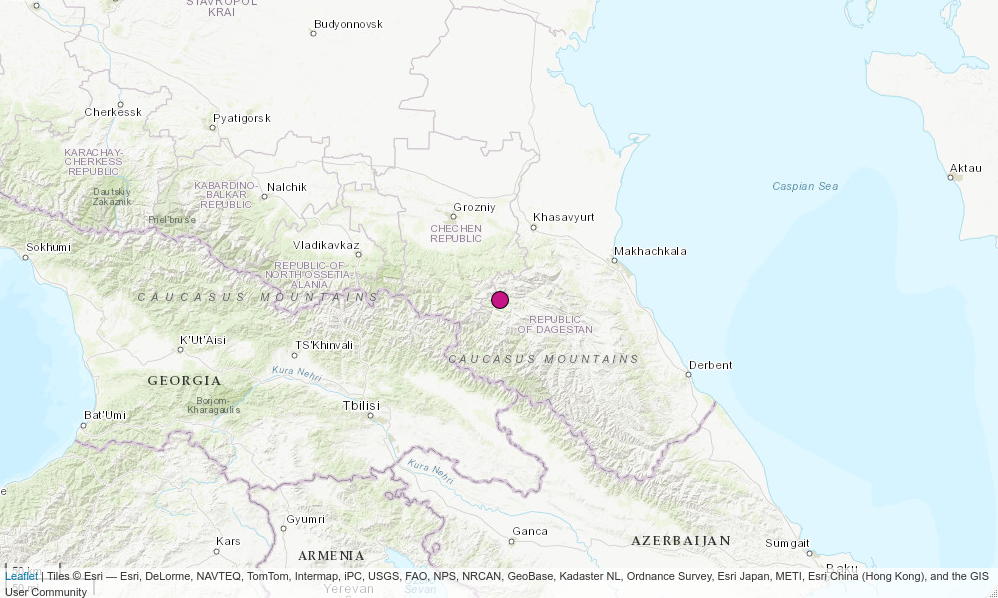
\includegraphics[scale=0.4]{images/globalmap.png}}
\end{figure}
\end{frame}

\section{Data}
\begin{frame}{Two dictionaries}

\begin{block}{\citep{saidovaabusov2012}}
    \begin{itemize}
        \item Compiled in the 2000s by a native speaker (M.G. Abusov) and an experienced linguist (P.A. Saidova)
        \item Mostly Botlikh with some notes on Miarso
    \end{itemize}
\end{block}

\pause

\begin{block}{\citep{alekseev2019}}
    \begin{itemize}
        \item Compiled in the 1960s / 1970s by a native speaker / philologist (X.G. Azaev) and later (in the 2000s) systematized by an experienced linguist (M.E. Alekseev)
        \item Subsequently edited by T.A. Maisak and scheduled for posthumous publication later this year
        \item Botlikh only % проверить Алексеева, возможно туда влезали миарсинские слова
    \end{itemize}
\end{block}
\end{frame}

\begin{frame}{Two dictionaries}

\begin{itemize}
    \item Dictionaries were compiled \textit{independently} of each other
    \item \textasciitilde{}8000 headwords \citep{saidovaabusov2012} vs. \textasciitilde{}9000 `words and expressions' \citep{alekseev2019} % посмотреть сколько входов мы вычислили
    \item No metadata on the speakers consulted
    \item Data from \citep{alekseev2019} was collected several decades earlier, but M.G. Abusov also consulted elderly speakers with the aim of collecting archaic vocabulary (p.c.)
    \pause
    \item At first glance, the two resources seemed to display variation
\end{itemize}

\end{frame}

\begin{frame}{Two dictionaries}

\begin{center}
    \textbf{Aim of the present investigation}\\
    Compare the two resources, see to what extent they overlap and diverge, and verify whether they display systematic variation\\
    ...
    \pause
    \vfill
    and \textit{hopefully}, explain the kind of variation we found\\ (idiolectal, diachronic, etc.) 
    
\end{center}

\end{frame}

\begin{frame}{Data}
Merge dictionaries (doc to xls table) through a painstaking process of unification (\href{https://github.com/agricolamz/}{George Moroz}).

\begin{figure}[h]
\centering
\fbox{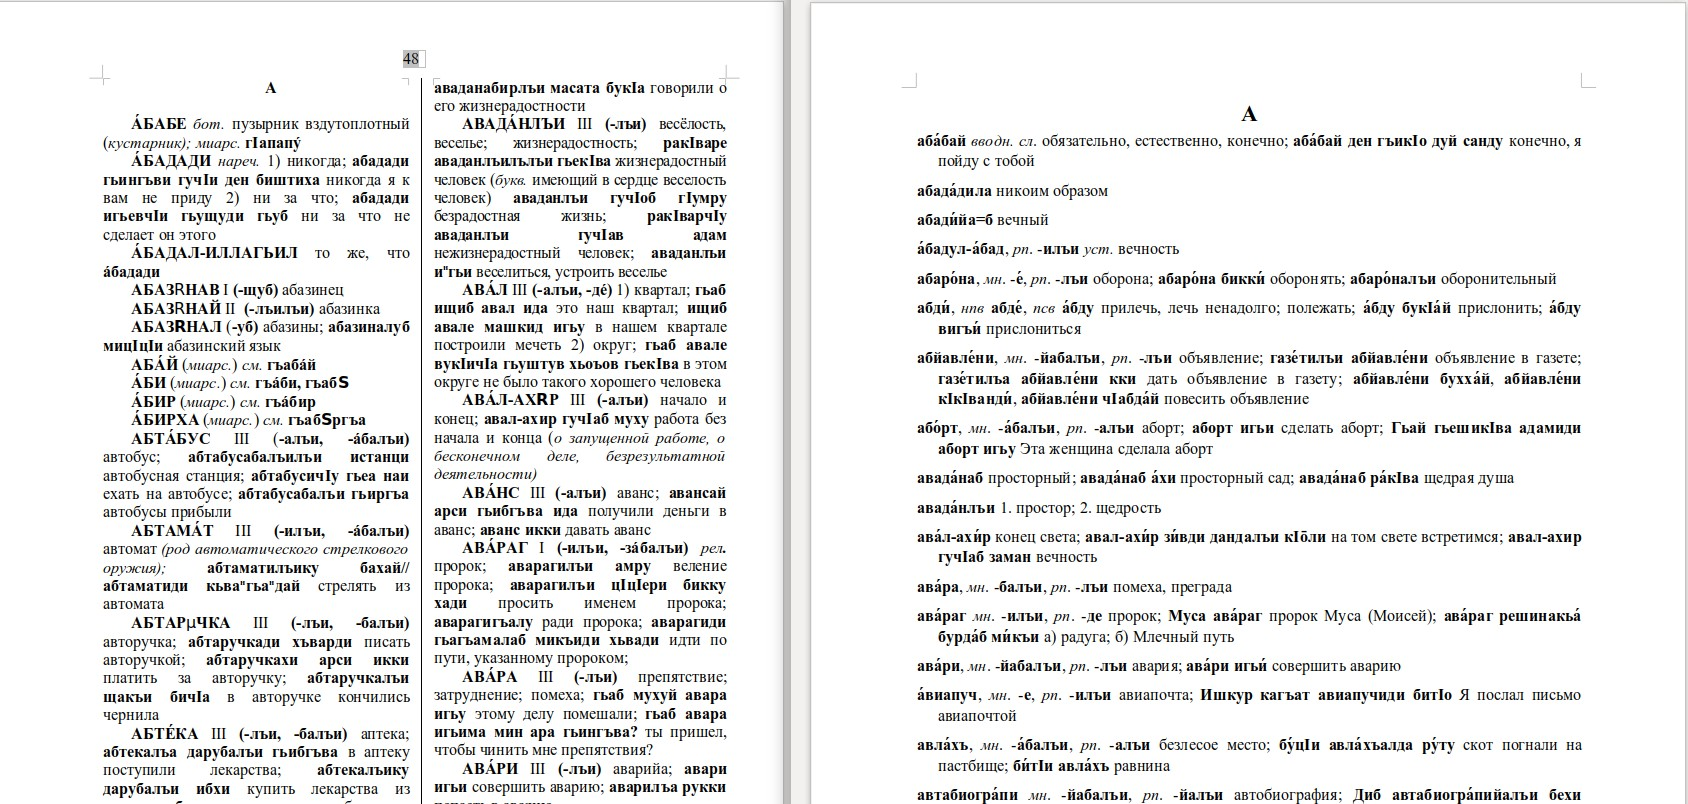
\includegraphics[scale=0.17]{images/dicts.jpg}}
\end{figure}
\end{frame}

\begin{frame}{Data}

Nouns (genitive, plural) and verbs (habitual and aorist)

\begin{figure}[h]
\centering
\fbox{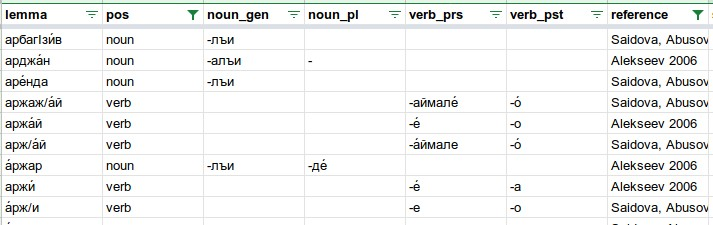
\includegraphics[scale=0.4]{images/table.jpg}}
\end{figure}
\end{frame}


\begin{frame}{Parameters}
\begin{itemize}
    \item Phonology: phoneme frequency, stress patterns, syllable structure
    \item Nominal morphology: formation of genitive case and plural forms
    \item Verbal morphology: formation of basic tenses
\end{itemize}
\end{frame}

\section{Variation}

\begin{frame}{Phonology}
    
\end{frame}

\begin{frame}{Nominal morphology}
Formation of the plural
\begin{itemize}
    \item A suffix is attached to the absolutive stem: \textit{na} `thing' < \textit{na-\textbf{baɬi}} `things'
    \item With stems ending in a consonant the vowel \textit{-a-} is often inserted before the suffix: \textit{majmalak}  `monkey' < \textit{majmalak-\textbf{a}-\textbf{baɬi}} `monkeys'
    \item With stems ending in a vowel alternation can occur: \textit{ruš\textbf{a}}  `tree' < \textit{ruš\textbf{i}-\textbf{baɬi}} `trees', \textit{sal\textbf{u}}  `tooth' < \textit{sal\textbf{a}-\textbf{baɬi}} `teeth', \textit{buraɬ\textbf{i}}  `pitcher' < \textit{buraɬ\textbf{a}-\textbf{baɬi}} `pitchers'
    \item Among the most common suffixes are: \textit{-baɬi} (and variants, e.g. \textit{-zabaɬi}, \textit{-maɬi}, etc.), \textit{-de}, \textit{-(w)e}
    %add more suffixes
\end{itemize}
\end{frame}

\begin{frame}{Nominal morphology}
Case declension (core cases)
\begin{itemize}
    \item I type --- the stem does not change when a suffix is attached (mainly stems ending in a vowel): \textit{bab\textbf{u}} `mom' < \textit{bab\textbf{u}-\textbf{ɬi}} (genitive)  
    \item II type --- case suffixes are attached to the oblique stem of the noun (mainly stems ending in a consonant, sometimes stems ending in a vowel): \textit{askar} `army' < \textit{askar-\textbf{a}-\textbf{ɬi}} (genitive), \textit{din} `religion' < \textit{din-\textbf{i}-\textbf{ɬi}} (genitive), \textit{ima} `father' < \textit{im\textbf{u}-\textbf{ɬi}} (genitive) 
% Contingency table - oblique stem + end of abs stem
\end{itemize}
\end{frame}

\begin{frame}{Nominal morphology}
\begin{itemize}
    \item Both dictionaries report both the \textbf{genitive} and the \textbf{plural} suffix
    \item We used this information to study the productivity of such suffixes, and to see whether the two dictionaries display variation
    \item We retrieved 2,965 nouns for A\&A, 2,952 for S\&A
    \item 1,072 pairs were present in both dictionaries and had information about inflectional forms
    \item The genitive suffix is almost always reported in both dictionaries: for all 1,072 words in S\&A, for 1,066 words in A\&A
    \item The plural is not reported for all words: for 571 words in S\&A, for 879 words in A\&A % such cases include nouns which are not normally used in the plural (e.g. abstract nouns), demonyms (because the plural form of the demonym is usually reported as a separate entry in the dictionary), masdars (Saidova&Abusov)
\end{itemize}
\end{frame}

\begin{frame}{Nominal morphology}
\begin{center} Variation: plural suffixes
\end{center}
\begin{figure}[h]
\centering
\fbox{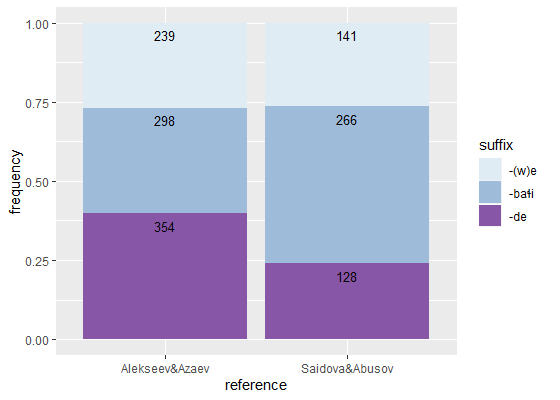
\includegraphics[height=6cm]{images/plural.png}}
\end{figure}
\end{frame}

\begin{frame}{Nominal morphology}
\begin{center} Variation: genitive in \textit{-aɬi} vs. \textit{-iɬi} with stems ending in a consonant
\end{center}
\begin{figure}[h]
\centering
\fbox{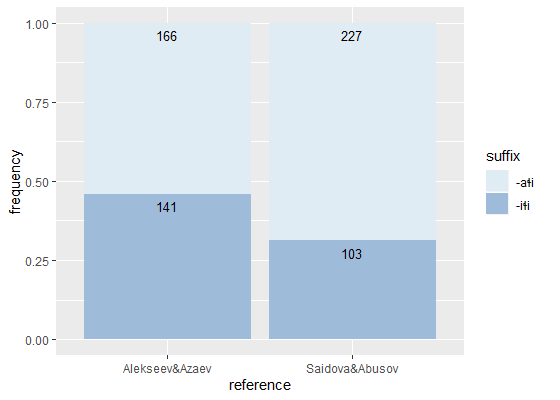
\includegraphics[height=6cm]{images/genitive.png}}
\end{figure}
\end{frame}

\begin{frame}{Nominal morphology}
Variation: examples
\begin{itemize}
    \item It seems that variation frequently involves loanwords: \textit{dakument} `document' < \textit{dakument-\textbf{aɬi}} (genitive, S&A) vs. \textit{dakument-\textbf{iɬi}} (genitive,A&A), \textit{birgadir} `foreman' < \textit{birgadir-\textbf{zabaɬi}} (plural, S&A) vs. \textit{birgadir-\textbf{de}} (plural, A&A)
\end{itemize}
\end{frame}

\begin{frame}{Verbal morphology}

\begin{itemize}
    \item We retrieved 1570 verbal entries for A\&A and 1475 for S\&A 
    \item Only 689 pairs were present in both dictionaries and had information about inflectional forms
    \pause 
    \item Botlikh has only one verb stem; suffixes are attached directly
    \item Infinitive and Aorist are indicative for conjugation:
    \pause

\begin{table}[h]
\caption{Basic verb inflection in Botlikh}
\label{tab:verbtense}
\label{tab:my-table}
\begin{tabular}{l|l|l|l}
          & \multicolumn{1}{c|}{infinitive} & \multicolumn{1}{c|}{present} & \multicolumn{1}{c}{past}        \\ \hline
Basic     & -i                              & -e                           & -a / -u / -iw                   \\
Causative & -a-j                            & mal-e / malih-e              & -o * \textless -a + u / malih-u \\
Derived   & -ɬi                             & b-ah-e                       & b-ah-i `become'                 \\
          &                                 & b-uk'-e                      & b-uk'-a `be'                   
\end{tabular}
\end{table}
\end{itemize}

\end{frame}


\begin{frame}{Verbal morphology}

% Synth. + Anal. + Mix forms

\end{frame}

\begin{frame}{Verbal morphology}

Synthetic forms: the past

% Aorist suffixes: words with -iw

\end{frame}

\begin{frame}{Verbal morphology}

Periphrastic forms: auxiliaries

% Aorist suffixes: words with -iw

\end{frame}


\begin{frame}{Verbal morphology}
\begin{itemize}
    \item Causative verbs have an infinitive suffix \textit{-aj}.
    \item Present tense is \textit{-aj male} in S\&A, \textit{-aj malihe} in A\&A (inf + aux).
    \item Past tense is simply \textit{-o} in S\&A, \textit{-o} or \textit{-aj malih-u} in A\&A.
    \item A form \textit{-aj malo} is attested once (!) in S\&A.
    \pause
    \item The bulk of material in A\&A was collected several decades earlier with respect to S\&A
\end{itemize}
\end{frame}


\begin{frame}{Verbal morphology}

% Contingency table infinitive + past

\end{frame}



\section{Summary}
\begin{frame}{Summary}
\begin{itemize}
    \item %So what did we learn from this?
    \pause
    \item Nominal morphology: 
    \pause
    \item Verbal morphology: verbs show diachronic and idiosyncratic variation
    \begin{itemize}
        \item The prs inflection of causatives has undergone morphologization in the newer dictionary
        \item 
    \end{itemize}
\end{itemize}
\end{frame}

\section{The end}
\begin{frame}{Всё}
% тут фотка красивая
\end{frame}

\section{Abbreviations}
\begin{frame}{Abbreviations}

\tiny{\printglossary}

\end{frame}

\section{References}
\begin{frame}{References}

\printbibliography

\end{frame}

\end{document}